I forbindelse med projektet er der blevet tænkt over en række metoder, som gør os i stand til at finde ind til vores problems kerne, og understøtte problemet i sin helhed.
Ud fra projektforslaget er det blevet fastsat at vores endelige løsning til problemet skal være en prototype af et program. Denne prototype skal være skrevet i C, men da problemstillingen omhandler SMS-beskeder, er det  SMS-mediets krav, som vi skal designe vores løsning efter.


Ud fra vores problem findes der en række interessenter, som påvirkes af denne problemstilling.
På den følgende brainstorm, ses hvordan disse interessenter fordeler sig, ud fra det initierende problem, og hvordan de forbindes til hinanden.

\begin{figure}[H]
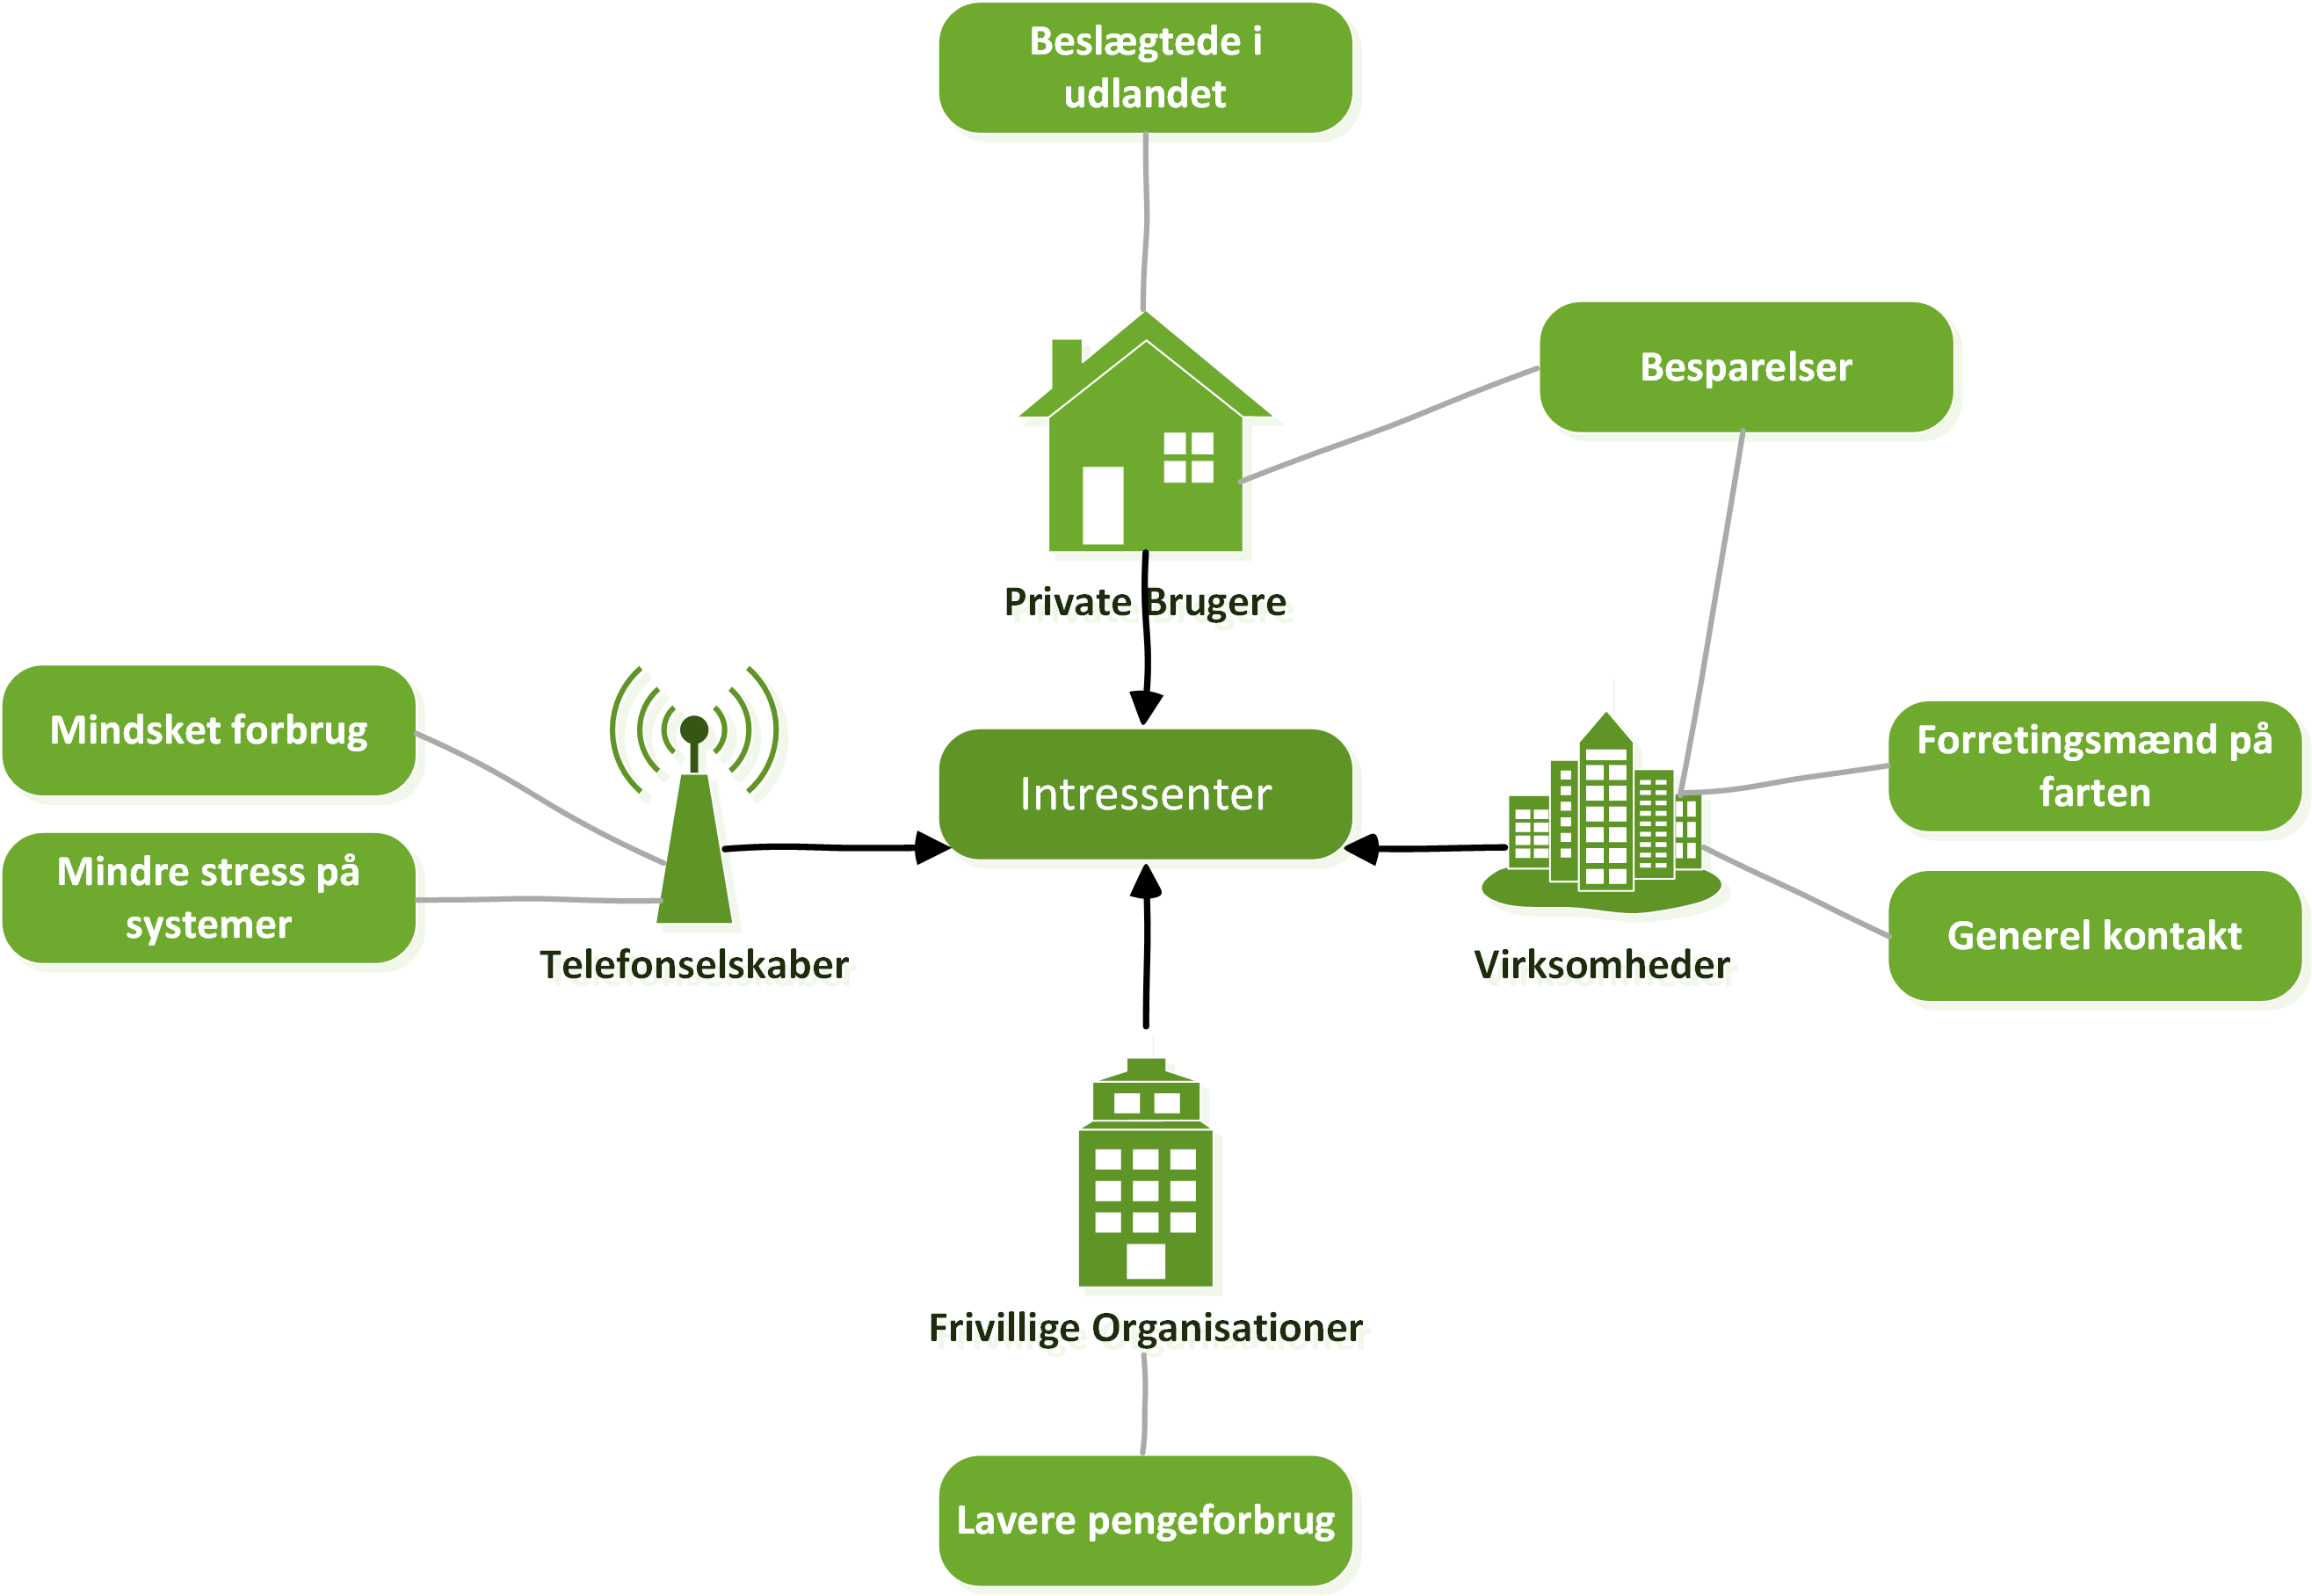
\includegraphics[width=\linewidth]{Billeder/Brainstormting.png}
\caption{Her ses hvordan interessenterne fordeler sig.}
\end{figure}

Denne brainstorm identificerer vores primære interessenter, som vil være vores hovedmålgruppe.
Man kan dele interessenterne ind i nogle grupper, henholdsvis: Private personer, internationale firmaer, frivillige organisationer og teleselskaber.
Hver af disse grupper har sin egen grund til at være interesseret i vores problemstilling, og derfor kan det også betyde, at der skal forskellige løsninger til at kunne løse problemstillingen, for hver forskellig interessent.


Ud fra vores problemstilling findes der en række data som kan være anvendelig i forhold til undersøgelsen af de førnævnte interessenter.


Viden om brugen af SMS'er hos de forskellige interessent grupper.
Det er vigtigt at finde ud af hvordan de forskellige interessenter bruger SMS'er som et medie. Med dette menes både hvor tit det bruges, men også i hvilken forbindelse og med hvem kommunikationen foregår.